\documentclass{article}
%\usepackage[top=30pt,left=30pt,right=30pt]{geometry}
\usepackage[german,english]{babel}
%\usepackage[utf8]{inputenc}
\usepackage{amsmath}
\usepackage{amssymb}
\usepackage{amsthm}
\usepackage{graphicx}
\usepackage{caption}
\usepackage{fontspec}
\usepackage{mdframed}
\usepackage{pxfonts}
\usepackage{wasysym}
\usepackage{framed}
\usepackage{xcolor}
\usepackage{makeidx}
\usepackage{csquotes}
\usepackage[pdfborder={0 0 0}]{hyperref}
\usepackage{stmaryrd}
\usepackage{titlesec}
\titleformat{\paragraph}{\normalfont\itshape}{}{}{}

\newcounter{lecref}[section]
\numberwithin{lecref}{section}
\setcounter{section}{-1}
\newcounter{exercises}

\newtheorem{theorem}[lecref]{Theorem}
\newtheorem*{Theorem}{Theorem}
\newtheorem{example}[exercises]{Example}
\newtheorem*{Example}{Example}
\newtheorem{definition}[lecref]{Definition}
\newtheorem*{Definition}{Definition}
\newtheorem{lemma}[lecref]{Lemma}
\newtheorem*{Lemma}{Lemma}
\newtheorem{claim}[lecref]{Claim}
\newtheorem*{Claim}{Claim}
\newtheorem{remark}[lecref]{Remark}
\newtheorem*{Remark}{Remark}
\newtheorem{algorithm}[lecref]{Algorithm}
\newtheorem*{Algorithm}{Algorithm}
\newtheorem{corollary}[lecref]{Corollary}
\newtheorem*{Corollary}{Corollary}
\newtheorem{proposition}[lecref]{Proposition}
\newtheorem*{Proposition}{Proposition}
\newtheorem{revision}{Revision}
\newtheorem*{Revision}{Revision}

\def\ifempty#1{\def\temp{#1} \ifx\temp\empty }

% useful control sequences for mathematical notation
\newcommand{\Abs}[1]{\left|#1\right|}
\newcommand{\Set}[1]{\left\{#1\right\}}
\newcommand{\SetDef}[2]{\left\{#1\,\mid\,#2\right\}}
\newcommand{\IP}[2]{\left\langle#1, #2\right\rangle}
\newcommand{\Norm}[1]{\left\|{\ifempty{#1}\cdot\else#1\fi}\right\|}
\newcommand{\Max}[1]{\max{\Set{#1}}}
\newcommand{\Min}[1]{\min{\Set{#1}}}
\newcommand{\Sup}[1]{\sup{\Set{#1}}}
\newcommand{\Powerset}[1]{{\mathbb P}(#1)}
\newcommand{\IntRange}[2]{#1, \dots\ifempty{#2}\else, #2\fi}

\def\vec2#1#2{\begin{pmatrix} #1 \\ #2 \end{pmatrix}}
\def\vec3#1#2#3{\begin{pmatrix} #1 \\ #2 \\ #3 \end{pmatrix}}
\newcommand{\noproof}[1]{A proof for Theorem~\ref{#1} is not provided.}
\newcommand{\dotted}[1]{\:\dot{#1}\:}  % dot has too little margin

% German translation
\newcommand{\dt}[1]{(dt. \enquote{\foreignlanguage{german}{#1}})}

% essential control sequences
%% \xRightarrow: \xrightarrow for \rightarrow like \xRightarrow for \Rightarrow
\makeatletter
\newcommand{\xRightarrow}[2][]{\ext@arrow 0359\Rightarrowfill@{#1}{#2}}
\makeatother

% typesetting settings
\parindent0pt
\setlength{\parskip}{.6em}
\setmainfont{CMU Serif Roman}

% TODO: span?
\DeclareMathOperator{\rank}{rank}
\DeclareMathOperator{\diag}{diag}
\DeclareMathOperator{\detm}{det}
\DeclareMathOperator{\perm}{perm}
\DeclareMathOperator{\sign}{sign}
\DeclareMathOperator{\degree}{deg}
\DeclareMathOperator{\im}{image}
\DeclareMathOperator{\ke}{kernel}
\DeclareMathOperator{\spec}{spec}
\DeclareMathOperator{\prop}{probability}
\DeclareMathOperator{\Hom}{Hom}
\DeclareMathOperator{\argmax}{argmax}
\DeclareMathOperator{\argmin}{argmin}
\DeclareMathOperator{\vol}{vol}  % volume
\DeclareMathOperator*{\bigtimes}{\vartimes}





\newcommand{\dateref}[1]{%
  \begin{mdframed}[backgroundcolor=gray!10,innerbottommargin=0pt,innertopmargin=0pt]
    \paragraph{\textit{$\downarrow$ This lecture took place on #1.}}%
  \end{mdframed}%
}

% metadata
\title{
  Optimization 1 \\
  \large{Lecture notes, University of Technology, Graz} \\
  based on the lecture by Bettina Klinz
}
\date{\today}
\author{Lukas Prokop}

\makeindex
\begin{document}

\maketitle
\tableofcontents

\section{Course}

\dateref{2019/03/04}

\begin{itemize}
	\item Lecture
	\begin{itemize}
		\item Monday, 12:15--14:00
		\item Tuesday, 16:15--18:00
	\end{itemize}
	\item First week, the practicals session will be used for the lecture
	\item Practicals will take place usually on Wednesday, 16:15--18:00 \\
		in exceptional cases on Thursday, 16:15--18:00
	\item 2 websites (work in progress):
		\begin{itemize}
			\item \url{http://www.math.tugraz.at/~klinz/optimvo} (list of literature)
			\item \url{http://www.math.tugraz.at/~klinz/optimue} (practicals mode, practicals exercises, additional content)
		\end{itemize}
	\item Two large topics in this lecture
		\begin{itemize}
			\item Linear optimization (linear target function, linear side conditions)
			\item Non-linear optimization without sub conditions (unconstrained non-linear optimization) \\
				where non-linear optimization denotes that the target function is non-linear
		\end{itemize}
	\item Be aware, that this class might be the lecture requiring previous results of classes the most.
	\item Advanced lecture in masters
		\begin{itemize}
			\item Lecture \enquote{Non-linear optimization} (includes nonlinear optimization with sub conditions)
		\end{itemize}
	\item Exam
		\begin{itemize}
			\item written + orally, in case of negotiation and few candidates only orally
			\item 1st date will be at the end of the semester, optionally in summer holidays
			\item 2 written exams for the practicals
		\end{itemize}
\end{itemize}

\subsection{Linear optimization}

We have already seen optimization problems in high school or previous semesters.
But, for example, handling constraints consisting of inequalities was tedious or trivial.
We consider more sophisticated techiques here.
In practice, linear models occur rarely. But they often provide a sufficient heuristic.

\subsection{Introduction and some examples for linear optimization models}

\begin{example}[Production planning model]
	\label{example:1}
	A factory can produce $n$ goods.
	The revenue per unit of good $j$ is given by $c_j$ units of money.
	Production is limited by restrictions, that result from constrained availability of staff, equipment and raw materials.
	Let $m$ denote the number of these resources and $b_i$ is the maximum availability of resource $i$ ($i = 1, \dots, m$).
	Let $a_{ij}$ with $1 \leq i \leq m$ and $1 \leq j \leq n$ denote the quantity of resource $i$ required to produce 1 unit of good $j$.
	Our goal is to maximize revenue with respect to the given constraints.

	\emph{Decision variable:} $X_j$ is the quantity of good $j$

	\[ \text{target function: } \max \sum_{j=1}^n C_j X_j \]
	\[ \text{ subject to (constraints) } \sum_{j=1}^n a_{ij} x_j \leq b_i \qquad i \in \Set{1, \dots, m} \]
	\[ \text{ with } x_j \geq 0 \qquad \text{ sign condition} \]

	Pay attention! We do not require $x_j \in \mathbb Z$. For $x_j \in \mathbb Z$ we get an integral linear program which is \emph{not} a linear programm! (this is a difficult subproblem of optimization)
\end{example}

\begin{example}[Mixture problem]
	\label{example:2}
	Consider $n$ kinds of raw materials. Our goal: We want to create a new material by mixing existing raw materials to reduce costs.

	\begin{Example}[Alloys]
		Consider $n$ different base alloys $L_1, \dots, L_n$.
		For each material we have the lead content in percent ($a_1, \dots, a_n$) and the costs per unit of weight ($c_1, \dots, c_n)$.
		We have to produce alloys with lead content $b \%$.
		The decision variable $X_j$ is given by the ratio of $L_j$.

		Formally, the problem can be defined as
		\[ \min{\sum_{j=1}^n c_j x_j} \text{ s.t. } \sum_{j=1}^n x_j = 1, \sum_{j=1}^n a_j x_j = b, x_j \geq 0 \]
		These are typical mixture constraints and they ensure a given lead content.
	\end{Example}
\end{example}

\begin{example}[Linear transportation problem]
  \label{example:3}
  Given $m$ firms, $n$ customers, $a_i$ is the offer by firm $i$ and $b_j$ is the demand by customer $j$.
  $c_{ij}$ are the transportation costs from firm $i$ to customer $j$.

  Find an admissible transportation plan with minimal costs.
  The decision variable $X_{ij}$ is the quantity of goods transported from firm $i$ to customer $j$.

  Formally,
  \[ \min{\sum_{i=1}^m \sum_{j=1}^n c_{ij} X_{ij}} \text{ s.t. } \sum_{i=1}^m X_{ij} = b_j, \sum_{j=1}^n X_{ij} = a_i, X_{ij} \geq 0 \quad j \in \Set{1, \dots, n}, i \in \Set{1, \dots, m} \]
\end{example}

\begin{Example}[Diet problem]
  The following problem has a strong historical background in optimization sciences:
  Stigler diet problem (in the year 1939) by Georg Stigler. 

  Given a list of 77 ingredients. Per ingredient we are given features such as calories and proteins.
  Find an optimal combination to minimize costs.

  His heuristic results were confirmed as almost optimal in 1947.
\end{Example}

In the following lectures, our goal will be:

\begin{itemize}
	\item Theory of linear optimization (Knowledge about fundamentals and background)
	\item Algorithmic solutions procedures: in the lecture we will discuss two procedures:
		\begin{itemize}
			\item Simplex process (G. Dantzig, 1947, in practice useful, no polynomial runtime)
			\item Inner point method (in practice useful, polynomial runtime)
		\end{itemize}
		Outside this lecture:
		\begin{itemize}
			\item Ellipsoid method: polynomial runtime, but in practice useless
		\end{itemize}
\end{itemize}

\section{Geometrical considerations of linear optimization}

\begin{Definition}
  Standard form of a linear program (canonical representation)
  \[ \max{z(x)} = z_0 + \sum_{j=1}^n c_j x_j \text{ such that } \sum_{j=1}^n a_{ij} x_j \leq b_i, X_j \geq 0 \qquad i \in \Set{1, \dots, m} \]
  In compact notation:
  \[ \max{z_0 + c^t x} \text{ s.t. } Ax \leq b, x \geq 0 \]
  typically $\max c^t x$.
  $z_0$ does not influence the result.

  \[ A = \begin{pmatrix} a_{11} & \dots & a_{1n} \\ \vdots & \ddots & \vdots \\ a_{m1} & \dots & a_{mn} \end{pmatrix} \qquad b = \begin{pmatrix} b_1 \\ \vdots \\ b_m \end{pmatrix} \qquad a_{ij} \in \mathbb R, b_i \in \mathbb R, c_j \in \mathbb R \]
\end{Definition}

\dateref{2019/03/05}

\begin{Revision}
	The canonical/standard form of a linear program is given by
	\[ \max c^t x \text{(} + \text{optionally } z_0 \text{) such that } Ax \leq b \qquad x \geq 0 \]
\end{Revision}

\begin{Remark}[Observation]
  Every arbitrary linear program (min/max of an affine linear function over a linear constraint) can be transformed into the canonical form above.
  \begin{enumerate}
  	\item The minimization over $c^t x$ corresponds to $-c^t x$ as maximization problem.
  	\item Constraints of form $\alpha^t x \geq b$ can be written as $-\alpha^t x \leq -\beta$.
  	\item A constraint of form $\alpha^t x = \beta$ can be written as $\alpha^t x \leq \beta$ with $\alpha^t x \geq \beta$. Or equivalently as $\alpha^t x \leq \beta$ with $-\alpha^t x \leq -\beta$.
  		\begin{Remark} \hfill
	  		\begin{itemize}
	  			\item Disadvantage: One constraint is transformed into two.
	  			\item In practice, the explicit handling of equality constraints should be preferred.
	  		\end{itemize}
  		\end{Remark}
  	\item Let $x_j$ not be restricted w.r.t. the sign. Write $x_j$ as $x_j = x_j^+ - x_j^-$ with $x_j^+ \geq 0$ and $x_j^- \geq 0$.
  		$x_j$ will be replaced by $x_j^+ - x_j^-$ with $x_j^+ \geq 0$ and $x_j^- \geq 0$.
  		\begin{Remark}
  			Disadvantage: Number of variables in increased.
  		\end{Remark}
  \end{enumerate}
\end{Remark}

\begin{Remark}[Terminology] \hfill{}
  \begin{itemize}
  	\item 2 points $u, v \in \mathbb R^n$ define a \emph{line} $G(u, v) = \SetDef{u + \lambda (v - u)}{\lambda \in \mathbb R}$. \index{Line}
  	\item A \emph{halfline} is formally given by $\SetDef{u + \lambda (v - u)}{\lambda \geq 0}$ \index{Halfplane}
  	\item A \emph{closed interval} (or \emph{segment}) is defined as $[u, v] = \SetDef{u + \lambda (v - u)}{\lambda \in [0, 1]}$ and
  		an \emph{open interval} is defined as $(u, v) = \SetDef{u + \lambda (v - u)}{\lambda \in (0, 1)}$. \index{Segment}\index{Open interval}\index{Closed interval}
  \end{itemize}
\end{Remark}

\begin{lemma}
	\label{lemma:1.1}
	\begin{itemize}
		\item An affine linear function $z_0 + c^t x$ takes up its maximum/minimum in segment $[u, v]$ in its end points $u$ or $v$.
		\item An affine linear function $z_0 + c^t x$ takes up its maximum/minimum on a half-line in the end points.
	\end{itemize}
\end{lemma}
\begin{proof}
	Left as an exercise to the reader (use parameter representation and insert it into the function)
\end{proof}

\subsection{Hyperplane and Halfspaces}

By the linear inequality $\alpha^t x \leq \beta$ ($\alpha \in \mathbb R^n, \beta \in \mathbb R$) with $\alpha \neq 0$ (zero vector) we define a \emph{closed halfspace}\index{Closed halfspace}.
\[ H_{\leq} \coloneqq \SetDef{x \in \mathbb R^n}{\alpha^t x \leq \beta} \]
Analogously we can define open halfspaces\index{Open halfspace}:
\[ H_{<} \coloneqq \SetDef{x \in \mathbb R^n}{\alpha^t x < \beta} \]
Hyperplane\index{Hyperplane}:
\[ H_{=} \coloneqq \SetDef{x \in \mathbb R^n}{\alpha^t x = \beta} \]
In $\mathbb R^2$, hyperplanes are halflines.
In $\mathbb R^3$, hyperplanes are halfplanes.

\begin{figure}[t]
	\begin{center}
		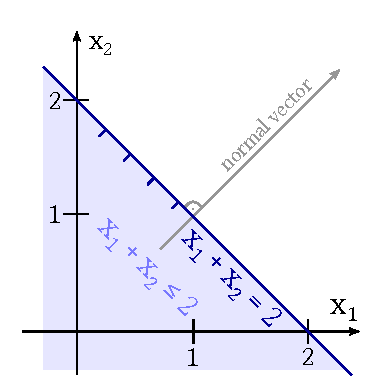
\includegraphics{img/02_constraint.pdf}
		\caption{Constraint $x_1 + x_2 \leq 2$ visualized in $\mathbb R^2$. To determine the halfplane (bright blue) resulting from the constraint, it helps to express the constraint with $x_2$ on the left-hand side: $x_2 \leq 2 - x_1$. Then determine $x_2$ for two different $x_1$ assuming an equality operator, e.g. $x_1 = 0$ with $x_2 = 2$ and $x_1 = 1$ with $x_2 = 1$. Then choose some large value $x_1$ and $x_2$ (e.g. $x_1 = 10$ and $x_2 = 10$). Does it satisfy $x_1 + x_2 \leq 2$? No, the halfplane containing $(10, 10)$ is not the one, we are looking for. Some people prefer to consider the normal vector. Sometimes dashes are used to mark the side of the considered halfplane.}
		\label{img:constraint-vis}
	\end{center}
\end{figure}

Possible cases for the position of lines $G(u, v)$ w.r.t. to the hyperplane $H = \SetDef{x}{\alpha^t x = \beta}$.
\begin{description}
	\item[Case 1] Line $G$ is contained in $H$ (denoted $G \subseteq H$) \\
		$\alpha^t u = \beta$, $\alpha^t (u - v) = 0$
	\item[Case 2] $G$ is parallel to $H$ \\
		$\alpha^t u \neq \beta$, $\alpha^t (u - v) = 0$
	\item[Case 3] $G$ intersects $H$ in one point $c$ \\
		$\alpha^t(u - v) \neq 0$
\end{description}

\begin{lemma}
  \label{lemma:1.2}
  If the line $G(u, v)$ is neither contained in halfplane $H = \SetDef{x}{\alpha^t x = \beta}$ nor in some open halfspace constrained by $H$, $G$ intersects the halfplane $H$ in one point.
\end{lemma}

\begin{Remark}[Observation]
  The parameter representation of a line is ambiguous. We can choose $u$ und $v$ wisely: $G(u, v), \overline{x} \in G$.
  We can always choose $u$ and $v$ such that $\overline{x} \in (u, v)$.

  Let $\overline{x} \in H_{<} = \SetDef{x \in \mathbb R^n}{\alpha^t x < \beta}$. If $G \subseteq H_<$, then $u, v \in H_<$.
  Otherwise, due to $\overline{x} \in G \cap H_{<}$, $G$ intersects the hyperplane $H = \SetDef{x \in \mathbb R^n}{\alpha^t x = \beta}$.

  Furthermore we can choose a representation $(u, v)$ such that $\overline{x} \in (u, v) \subseteq H_{<}$ and $v \in H_{=}$.
  This can be generalized to multiple halfspaces.
\end{Remark}

\begin{Definition}
  A \emph{polyhedron}\index{Polyhedron}\dt{Polyeder} is the intersection of finitely many halfspaces.
  A bounded polyhedron is also called \emph{polytope}\index{Polytope}.

  % TODO Boundaries of a polyhedron in $\mathbb R^2$, A polytope in $\mathbb R^2$ 
\end{Definition}

\begin{Remark}[Observation]
  The admissible set $P(A, b)$ of the linear program (given in the previous revision) is a polyhedron.
\end{Remark}

\begin{lemma}
  \label{lemma:1.3}
  Halfspaces and thus also polyhedrons are convex sets.
\end{lemma}

Furthermore affine-linear functions are convex \emph{and} concave.
Linear optimization is a special case of convex optimization minimizing a convex function over a convex set.
The neat property of such convex optimization tasks is that local and global minima/maxima collapse (just like in the linear case).

\paragraph{Geometric illustration for $n=2$}
$n=2$ means that we consider $2$ variables.
\[ \max c_1 x_1 + c_2 x_2 \qquad a_{i1} x_1 + a_{i2} x_2 \leq b_i \quad i = 1, \dots, m \qquad x_1, x_2 \geq 0 \]

\begin{figure}[t]
	\begin{center}
		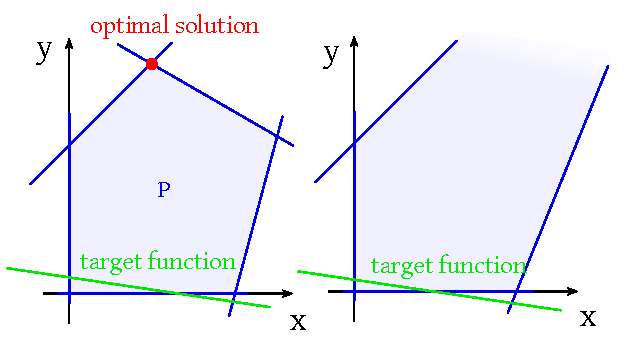
\includegraphics{img/01-bounded-set.pdf}
		\caption{Bounded (left) and unbounded (right) sets. The unbounded set does not have an optimal solution.}
		\label{img:boundedness}
	\end{center}
\end{figure}

\begin{Remark}[Observation]
  Optimal solutions occur at vertices of the set (intersection of two constraints). Compare with Figure~\ref{img:boundedness}.
\end{Remark}

This approach provides a graphical solution method for linear programs with 2 variables.

The generic geometric consideration of a polyhedron is
\[ P = \SetDef{x \in \mathbb R^n}{Ax \leq b} \qquad A \in \mathbb R^{m \times n} \]
Without loss of generality, we assume all row vectors $a_i$ of $A$ are non-zero.
\[ H_i \coloneqq \SetDef{x \in \mathbb R^n}{a_i^t x = b_i} \qquad \text{i-th halfplane} \quad i = 1, \dots, m \]

Let $I \subseteq \Set{1, \dots, m}$. Consider
\[ \hat H_I \coloneqq \bigcap_{i \in I} H_i = \SetDef{x \in \mathbb R^n}{a_i^t x = b_i \text{ for } i \in I} \qquad \text{ affine subspace of } \mathbb R^n \]
If $\hat H_I \cap P \neq P \neq \emptyset$, then this set is called \emph{face}\index{Face} of $P$.
The face of $P$ is called minimal\index{Minimal face}, if it does not contain any other face properly.

\begin{Example}
	A cube in $\mathbb R^3$ has 27 faces:
	\begin{itemize}
		\item The cube itself, $I = \emptyset$
		\item 6 faces, $I = \Set{1}, I = \Set{2}, \dots, I = \Set{6}$
		\item 12 face edges, $\Abs{I} = 2$
		\item 8 vertices, $\Abs{I} = 3$
	\end{itemize}
\end{Example}

\begin{Example}[Faces in the left subfigure in Figure~\ref{img:boundedness}]
	11 faces in total (5 vertices of dimension 0, 5 with dimension 1, 1 with dimension 2)
\end{Example}

More formally:
Let $P$ be described by a hyperplane $H_i$ ($a_i^t x = b_i$).
Let $S \subseteq \mathbb R^n, S \neq 0$.
\begin{Definition}
	$I(S) \coloneqq \SetDef{i \in \Set{1, \dots, m}}{S \subseteq H_i}$
\end{Definition}
For $S = \Set{x_0}$, we write $I(x_0)$ instead of $I(\Set{x_0})$.

\begin{Definition}
	\[ L(S) \coloneqq \SetDef{x}{a_i^t x = b_i, i \in I(S)} \]
	is the smallest affine subspace containing $S$.
	For a non-empty $S$, $S$ is a face iff $S = L(S) \cap P$.

	If $S$ is a minimal face, then $S = L(S)$ ($L(S)$ is then a part of the polyhedron).
\end{Definition}

\begin{Definition}[Dimension of a face]
	\[ \dim{S} \coloneqq \dim{L(S)} \]
	so the dimension of the smallest affine subspace containing $S$.
\end{Definition}
\begin{Definition}[Vertex]
	A vertex is a face of dimension $0$.
\end{Definition}
\begin{Remark}
	For polyhedron, the vertex term from above is an alternative definition for the vertex term for convex sets (the terms correspond).
\end{Remark}
\begin{Remark}
	A circle has infinitely many vertices; not none.
\end{Remark}

Let $S$ be convex set in $\mathbb R^n$.
$x$ is called vertex of $S$ if it is not possible to represent $x$ as $x = y + (1 - \lambda) z$ with $y, z \in S, y \neq z, \lambda \in [0,1]$.

\dateref{2019/03/06}

% TODO Problem with two parallel boundaries.

Not every polyhedron has vertices. For example, if the boundaries are given as two parallels, then no vertices can be identified.

\begin{Remark}
	The problem with two parallels is not representable in canonical form.
\end{Remark}

\begin{Definition}
	\index{Acute polyhedron}
	A polyhedron \emph{with} vertices is called \emph{acute}.
\end{Definition}

A vertex is a minimal face.
A face results as unique solution of the corresponding equation system.
\[ a_i^t x = b_i \qquad \forall i \in I(z) \]
If face $S = L(\overline{x}) \cap P$ for $\overline{x} \in \overline{P(A, b)} \eqqcolon P$ has dimension $\geq 1$ (hence no vertex),
then you can let some line $G$ pass through $\overline{x}$ that lies in $L(\overline{x})$.

$\overline{x}$ lies in the intersection of open halfspaces $\SetDef{x}{a_i^t x < b_i, i \not\in I(\overline{x})}$.
Thus we can provide a representation of line $G$ passing through two points $c$ and $d$ with $c, d \in S, \overline{x} \in (c, d)$.

Assume the halfspace with end point $\overline{x}$ in direction $d$ is bounded by some of the constraining hyperplanes of these open halfspaces.
Then $d$ can be chosen as the closest intersection point of the line with one of these hyperplanes $H_i$ for $i \not\in I(\overline{x})$.
\[ \implies \Abs{I(d)} > \Abs{I(\overline{x})} \qquad \implies \dim{L(d)} < \dim{L(\overline{x})} \]

Analogously, the same applies to the constraint by the halfline with end point $\overline{x}$ and in direction $c$.
$\dim{L(c)} < \dim{L(\overline{x})}$. Step by step, we can reduce the dimension to end up with a vertex.

\begin{theorem}[Statement about acute-angled polyhedrons]
	\label{theorem:1.4}
	\begin{enumerate}
		\item A non-empty polyhedron is acute iff it does not contain any line.
		\item Every face of an acute polyhedron contains one vertex.
		\item A polyhedron has (at most) finitely many vertices.
	\end{enumerate}
\end{theorem}
\begin{proof}
	\begin{enumerate}
		\item[1a.]
			Assume $P$ does not contain any lines. Let $x_0 \in P$ ($P \neq 0$).
			If $x_0$ is a vertex, then $P$ is acute. If $x_0$ is not a vertex, then consider the face $S \coloneqq L(x_0) \cap P$.
			Then $\dim{S} \geq 1$ holds true. Now we use the idea, that was sketched above right before the theorem.

			We choose a line $G(c, d) \subseteq L(x_0)$ where $c$ and $d$ are chosen as described before.
			Because $P$ does not contain a line, $S$ also does not contain any.
			Without loss of generality, we assume that the halfline with end point $x_0$ in direction $d$ is bounded and thus $\dim{L(d)} < \dim{L(x_0)}$.
			If $d$ is not a vertex, repeat this construction with some new $x_0 = d$.

			In every step, we are losing at least one dimension. After at most $n$ steps, we are going to have a vertex.
		\item[1b.]
			Let $P$ be acute, then $P$ has a vertex.
			Choose a vertex $\overline{x}$ and $n$ inequalities with maximum row rank.
			$I \subseteq I(\overline{x})$, submatrix $A_I$ of $A$ has $\rank(A_I) = n$.

			Assume there exists a line $G(u, v)$ with $u \neq v$, that in entirely contained in $P$.
			The inequalities $A_I u + \lambda \cdot A_I (v - u) \leq b_I$ must be true for all $\lambda \in \mathbb R$.

			Because $\lambda$ is unbounded, it should be true that $A_I(v - u) = 0$ where $A_I$ is a matrix of full rank.
			So $v - u = 0 \implies v = u$. This is a contradiction.
		\item[2.]
			A face $S$ of an acute polyhedron $P$ cannot contain any line because $S \subseteq P$ und $S$ is itself a polyhedron.
			By the first statement, $S$ has one vertex.
		\item[3.]
			Let $P$ be described by some $m \times n$ matrix $A$.
			$\Set{1, \dots, m}$ has only finitely many subsets.
			Thus we have only finitely many faces.
			\[ \leq {m \choose n} \text{ vertices} \]
	\end{enumerate}
\end{proof}

\begin{Remark}
  By Theorem~\ref{theorem:1.4}, it is immediate that non-empty polyhedrons, that result from linear programs in canonical form,
  $P = \SetDef{x \in \mathbb R^n}{Ax \leq b, x \geq 0}$ are always acute. So it has at least one vertex
  (because the set $\SetDef{x \in \mathbb R^n}{x_i \geq 0, i \in \Set{1, \dots, n}}$ does not contain a line).
\end{Remark}

\subsubsection{Fundamental theorem of Linear Optimization}

\begin{theorem}[Fundamental theorem of Linear Optimization]
  \label{theorem:1.5}
  \begin{enumerate}
  	\item
	  If an affine-linear function $z(x)$ takes up its maximum/minimum in a polyhedron $P$ in $\overline{x} \in P$, then also in all points of face $S = L(\overline{x}) \cap P$.
	\item
	  Especially the optimum is taken up in a vertex of $P$, if $P$ is acute.
  \end{enumerate}
\end{theorem}

\begin{proof}
	\begin{enumerate}
	\item
	  Let $\overline{x}$ be a maximum (analogously for minima) and let $y \neq \overline{x}$ be another point at $S$.
	  Then the line $G \coloneqq G(\overline{x}, y)$ in $L(\overline{x})$.
	  For $G$ there exists a representation $G = G(c, d)$ with $c, d \in P, \overline{x} \in (c, d)$.
	  By Lemma~\ref{lemma:1.1} the affine-linear function $z(x)$ takes up its maximum in line segment $[c, d]$ in $c$ or $d$.
	  Without loss of generality, we assume its maximum in $c$.
	  Thus $z(c) \geq z(\overline{x})$, because $\overline{x} \in (c, d)$.

	  On the other hand, we have $z(\overline{x}) \geq z(c)$, because $c \in P$ and the maximum is reached in $\overline{x}$.

	  Thus $z(c) = z(\overline{x})$. Hence, $z(x)$ is constant in $G$ and therefore $z(y) = z(\overline{x})$.
	  $y$ was chosen arbitrarily, then $z$ is constant at face $S$.
	\item
	  Follows by Theorem~\ref{theorem:1.4} (b).
	\end{enumerate}
\end{proof}

The polyhedron for linear programs in canonical form are empty or acute (have vertices).
The Fundamental theorem of Linear Optimization followingly states that for such linear programs (and thus any linear program becausc every linear program can be represented in canonical form) it suffices to investigate all vertices.

\begin{corollary}
	\label{corollary:1.6}
	If $\max\Set{c^\bot x: x \in P}$ has a linear optimization solution $x^*$, then $c^t x^* = \max\Set{c^t x: x \in V(P)}$ where $V(P)$ is the set of vertices of $P$.
\end{corollary}

Thus we retrieve a finite method for linear programs:
Determine all vertices and filter the vertex optimizing the target function.

\begin{Remark}[Disadvantage]
	Because there are exponentially (in $n$ and $m$) many vertices in general,
	there is no practically useful method of this idea.
\end{Remark}

\section{The generic Simplex Method}
\label{section:2}

The Simplex Method goes back to George Dantzig (1947).
The method relies on the Fundamental theorem of Linear Optimization and tries to find an optimal vertex.
It utilizes convexity to claim a local minimum as global one. Thus for a given vertex $x^*$, any adjacent vertex (reachable by one edge) has a worse target function value.

The basic idea is:
\begin{enumerate}
	\item Determine an initial vertex $x$ (if none exists, the polyhedron is empty because we utilize the canonical form).
	\item Test whether $x$ is a local optimum. Consider the edges starting from $x$ (they are either unbounded or lead to adjacent vertices).
	\item If $x$ is a local optimum, then stop.
	\item Otherwise either an unbounded problem is given or we replace $x$ by some adjacent vertex with a better target function value.
	\item Iterate this process.
\end{enumerate}

This process is necessarily finite, because there are only finitely many vertices.
This process gives rise to the generic Simplex algorithm:
\begin{enumerate}
	\item Choose an arbitrary vertex $x$ of $P$ as initial vertex. If none exists ($P = \emptyset$), then stop.
	\item While there exists some edge $k$ starting from $x$ increasing along the target function value, do
		\begin{enumerate}
			\item Choose such an edge
			\item If $k$ is not a halfline of our polyhedron $P$ then
			\begin{enumerate}
				\item substitute $x$ by edge $\tilde x$ at the other end of $k$
			\end{enumerate}
			else stop, as the problem is unbounded
		\end{enumerate}
	\item Return vertex $x$
\end{enumerate}

\dateref{2019/03/11}

Our next goal is to implement of this algorithmic idea algebraically.

\begin{Remark}[Observation]
  It is difficult to transform inequality systems of form $Ax \leq b$.
\end{Remark}

Transformation of an inequality system: \\
Canonical form $\max\Set{c^\bot x \text{ s.t. } Ax \leq b_1, x \geq 0}$ with $x \in \mathbb R^n, b \in \mathbb R^m, c \in \mathbb R^n, A \in \mathbb R^{m \times n}$.

Polyhedron $P = \SetDef{x \in \mathbb R^n}{Ax \leq b, x > 0}$.

Introduction of auxiliary variables $y_i$ (slack variables) \dt{Schlupfvariable}.
$y = b - Ax$ in vector notation.
$y_i = b_i - a_{i1} x_1 - \dots - a_{in} x_n \quad i = 1, \dots, m$.

Every point $x \in \mathbb R^n$ corresponds to exactly one point $\begin{pmatrix} x\\y \end{pmatrix} \in \mathbb R^{n + m}$.

Polyhedron $P$ $\to$ polyhedron $\tilde P = \SetDef{\begin{pmatrix} x\\y \end{pmatrix} \in \mathbb R^{m + n}}{Ax + y = b, x, y \geq 0}$.
The polyhedron structure is retained in such a way that dimensions of faces are preserved and vertices will become vertices.

The following correspondence will become useful:
\[ x_{n+1} \coloneqq y_1 \qquad x_{n+2} \coloneqq y_2 \qquad \dots \qquad x_{n+m} \coloneqq y_m \]
This provides a uniform naming of variables.

This results in the following representation, we call \emph{normal form}\index{Normal form of an optimization problem}
\[ \max{c_1 x_1 + \dots + c_n x_n + c_{n+1} x_{n+1} + \dots + c_{n+m} x_{n+m}} \]
subject to
\[
	\begin{array}{cccccc}
		a_{11} x_1 &+ \dots &+ a_{1n} x_n &+ x_{n+1} &           &= b_1 \\
		a_{11} x_1 &+ \dots &+ a_{1n} x_n &          &+ x_{n+1}  &= b_2 \\
		a_{11} x_1 &+ \dots &+ a_{1n} x_n &          & \vdots    & \\
		a_{m1} x_1 &+ \dots &+ a_{mn} x_n &          & \vdots    &= b_m \\
		       x_1 &, \dots, &x_{m+n}  &          &           &\geq 0
	\end{array}
\]
We agree on $c_{n+1} = \dots = c_{n+m} = 0$.

In the following, we will also denote the previous coefficient matrix with $A$.
This $A$ results from the canonical form and a $m \times n$ unit matrix $I$.
\[ \left(\begin{array}{c|c} A_{\text{canonical}} & I \end{array}\right) \]

\begin{Example}[Canonical form]
	\[ \max x_1 + x_2 \]
	s.t.
	\begin{align*}
		x_1 + 2x_2 &\leq 4 \\
		2x_1 - x_2 &\leq 3 \\
		x_2 &\leq 1 \\
		x_1, x_2 &\geq 0
	\end{align*}
\end{Example}

\begin{Example}[Normal form]
	\[ \max x_1 + x_2 \]
	s.t.
	\begin{align*}
		x_1 + 2x_2 + x_3 &= 4 \\
		2x_1 - x_2 + x_4 &= 3 \\
		x_2 + x_5 &\leq 1 \\
		x_1, x_2, \dots, x_5 &\geq 0
	\end{align*}
\end{Example}

\begin{Remark}
	In the following, we assume a linear program in normal form.
	$A$ is a $m \times (m + n)$ matrix for which we assume that it has full row rank $\operatorname{rank}(A) = m$.
\end{Remark}

In a similar way, $P$ denotes the polyhedron corresponding to our system $Ax = b, x > 0$.
Let $J \subseteq \Set{1, \dots, m+n} \to (J(1), J(2), \dots, J(k))$ be a map to index vectors where $J$ is an index set $\Abs{J} = K$.

Be aware that we implicitly switch between sets and tuples.

Our next goal is to introduce the terms basis, basis solution, non-basis.

\begin{Definition}
  A submatrix $A_B$ of $A$ with $A_{B} = (A_{B(1)}, \dots, A_{B(m)})$ and $\rank{A_B} = m$ (thus the m columns of $A_B$ are linear independent)
  is called \emph{basis matrix}\index{Basis matrix} and $B$ is called \emph{basis}\index{Basis}. Here we assume that $A_B$ is regular.
\end{Definition}

The remaining columns of $A$ are summed up in index vector $N$.
\[ \text{matrix } A_N = (A_{N(1)}, \dots, A_{N(n)}) \text{ where } N = \Set{1, \dots, m+n} \setminus B \]
$N$ is called \emph{non-basis}\index{Non-basis} and considered as set. $A_N$ is called \emph{non-basis matrix}\index{Non-basis matrix}.

We call $x_j$ with $j \in B$ \emph{basis variable}\index{Basis variable} and $x_j$ with $j \in N$ \emph{non-basis variable}\index{Non-basis variable}.

The following compact notations are practical: \\
\begin{tabular}{ccl}
	$x_B$ & \dots & vector of basis variables \\
	$x_N$ & \dots & vector of non-basis variables \\
	$c_B$ & \dots & vector of cost-coefficients $c_j$ for $j \in B$ (basis variable) \\
	$c_N$ & \dots & vector of cost-coefficients $c_j$ for $j \in N$ (non-basis variable)
\end{tabular}
\[ \max c^t x \qquad Ax = b, x \geq 0 \]
\[ \implies \max c_B^t x_B + c_N^t x_N \qquad A_B x_B + A_N x_N = b; x_B, x_N \geq 0 \]
We can write it as,
\[ c = (c_B, c_N) \quad x = (x_B, x_N) \quad A = (A_B, A_N) \]

\begin{Definition}
  A vector $x \in \mathbb R^{m + n}$ is called \emph{basis solution}\index{Basis solution} of a linear optimization problem in normal form ($\max\SetDef{c^t x}{Ax = b, x \geq 0}$), if there exists some basis $B$ with $A_B x_B = b$ and $x_N = 0$ (remark: $x_B = A_B^{-1} b$).

  A basis solution is called \emph{admissible}\index{Admissible solution} if $x_B \geq 0$. In this case, $B$ is called \emph{admissible basis}\index{Admissible basis}.
\end{Definition}

A basis solution is called \emph{degenerate}\index{Degenerate basis solution}, if there exists some $i$ with $x_{B(i)} = 0$.
Otherwise $x_B$ is called non-degenerate. Analogously we define \emph{degenerate bases}\index{Degenerate basis} and \emph{non-degenerate bases}\index{Non-degenerate basis}.

\begin{Remark}
	A basis solution $x$ is in polyhedron $P$, if it is admissible.
\end{Remark}

For the generic Simplex method, we go from vertex to vertex and thus from admissible solution to admissible solution.

\begin{Example}
	$N = (1, 2)$. So, non-basis variables are $x_1, x_2$ \\
	$B = (3, 4, 5)$. So, basis variables are $x_3, x_4, x_5$.

	The corresponding basis solution $(0, 0, 4, 3, 1)$.
\end{Example}

\[ N = (1, 5) \qquad B = (2, 3, 4) \]
is the corresponding basis solution.

Solve the system:
\[ \begin{pmatrix} 2 & 1 & 0 \\ -1 & 0 & 1 \\ 1 & 0 & 0 \end{pmatrix} \begin{pmatrix} x_2 \\ x_3 \\ x_4 \end{pmatrix} = \begin{pmatrix} 4 \\ 3 \\ 1 \end{pmatrix} \]
\begin{align*}
	2x_2 + x_3 &= 4 \\
	-x_2 + x_4 &= 3 \\
	x_2        &= 1
\end{align*}
So $x_3 = 2$ and $x_4 = 4$
\[ (0, 1, 2, 4, 0) \]
is admissible and non-degenerated.

\[ B = (1, 2, 3) \qquad N = (4, 5) \]
\[ B = (1, 2, 4) \qquad N = (3, 5) \]
\[ B = (1, 2, 5) \qquad N = (3, 4) \]
all lead to $x = (2, 1, 0, 0, 0)^t$ (admissible, degenerated).

\begin{Remark}[Here be dragons]
	To some non-degenerate basis solution, there exists exactly one basis.
	This does not hold true for degenerated basis solutions.

	The same vertex of the polyhedron corresponds to several bases in case of degeneration.
\end{Remark}

\begin{theorem}
	\label{theorem:2.1}
	The admissible basis solutions correspond to the vertices of the polyhedron, vice versa.
	If the basis solution is non-degenerated, then the corresponding basis is uniquely determined.
\end{theorem}

\begin{proof}
	\begin{enumerate}
	\item
		The basis solution $\tilde x$ (for basis $B$ and non-basis $N$) maps [by the definition of the basis solution] to $\tilde x_N = 0$ and $\tilde x_B$ is the unique solution of $A_B \tilde x_B = b$ ($Ax = b$).
		\[ \Set{\tilde x} = \SetDef{x}{x_N = 0} \cap \SetDef{x}{Ax = b} \]
		If $\tilde x$ is an admissible basis solution, then $\tilde x_B \geq 0$ and thus $\tilde x \geq 0$ and thus $\tilde x \in P$.
		Hence $\tilde x$ is a vertex of $P$.
	\item
		Let $\hat x$ be a vertex of $P$. Then the sign conditions must be satisfied and $\hat x$ is not uniquely defined by $m+n$ equations.
		Hence $\left\{ \begin{array}{c} n \\ x \end{array} \right\} = \SetDef{x}{x_N = 0} \cap \SetDef{x}{Ax = b}$ with $N \subseteq \Set{1, \dots, m+n}$.
		$A_B$ must be regular. $\hat x$ is basis solution.
	\item
		In some non-degenerated basis solution, there are exactly $m$ components $\neq 0$.
		$B$ is uniquely defined and thus $N$.
	\end{enumerate}
\end{proof}

Theorem~\ref{theorem:2.1} allows us to use basis solutions to implement the Simplex method numerically/algebraically.

\begin{Remark}
  Let a linear program in normal form be given. We assume it was transformed from the canonical representation.
  With $N = (1, \dots, n)$ and $B = (n+1, \dots, n+m)$ for $b \geq 0$, we always get one admissible basis solution
  $x \: \begin{pmatrix} x_N = 0 \\ x_B = b \end{pmatrix}$. This corresponds to the origin in the coordinate system of the canonical form.
  It can be used as initial guess in the Simplex method. For the other cases, we are still looking for an approach.
\end{Remark}

Now let $B$ be a fixed basis and $N$ is the corresponding non-basis.
\[ Ax = b \iff A_B x_B + A_N x_N = b \qquad A_B \text{ regular} \]
\[ x_B = A_B^{-1} (b  A_N x_N) = \underbrace{A_B^{-1} b}_{\coloneqq \tilde b} - \underbrace{A_B^{-1} A_N}_{\tilde A_N} x_N \]
\[ \tilde b \coloneqq A_B^{-1} b \qquad \tilde A_N = A_B^{-1} A_N \]
\[ x_B = \tilde b - \tilde A_N x_N \]

Polyhedron P:
\[ x_B = \tilde b - A_N x_N \qquad x_B, x_N \geq 0 \]
where the basis variables are represented by the non-basis variables.
This is the reduced representation wrt. $(BN)$.

Representation of form:
\[ x_{B(i)} = t_{i_0} + \sum_{j=1}^n t_{ij} x_{N(j)} \qquad i = 1, \dots, m \]
where $t_{ij}$ are the representation coefficients $t_{ij}$ with $i = 1, \dots, m$ and $j = 0, \dots, n$.

Projection of the polyhedron in the space of independent variables (non-basis variables).

We retrieve the canonical form representation in this space
\[ \tilde A_N x_N \leq \tilde b \qquad x_N \geq 0 \]

\begin{Example}[continued]
	\[ N = (1, 5) \qquad B = (2, 3, 4) \]
	\begin{align*}
		x_3 &= 2 - x_1 + 2 x_5 \\
		x_4 &= 4 - 2x_1 - x_5 \\
		x_2 &= 1 - x_5
	\end{align*}
\end{Example}

We want to insert this new representation into the target function.
\begin{align*}
	z(x) = z
		&= z_0 + c^t x = z_0 + c_B^t x_B + c_N^t x_N \\
		&= \underbrace{(z_0 + \underbrace{c_B^t A_B^{-1} b}_{\text{constant}})}_{\tilde z_0} - \underbrace{(c_B^t A_B^{-1} A_N X_N + C_N^t x_N)}_{+ (c_N^t - c_B^t A_B^{-1} A_N) x_N} \\
		&= \tilde z_0 + \tilde c_N^t x_N
\end{align*}
with $\tilde c_N^t = c_N^t - c_B^t \underbrace{A_B^{-1} A_N}{\tilde A_N}$. $\tilde c_N$ is called \emph{reduced cost coefficients}\index{Reduced cost coefficients}. Later, $\tilde z_0$ and $\tilde c_N$ will become the 0-th row of the coefficient tableau.

\dateref{2019/03/12}

\begin{Revision}
	\[ z \coloneqq t_{00} + \sum_{j=1}^n t_{0j} X_{N(j)} \]
	as 0-th row of the tableau.
	\begin{Example}
		\[ N = (1, 5) \qquad B = (2, 3, 4) \]
		\[ \max x_1 + x_2 = 1 + x_1 - x_5 \]
		Let $x_2 = 1 - x_5$.
		Representation of the target function in the space of non-basis variables.
	\end{Example}
\end{Revision}

\subsection{Sufficient optimality criterion for basis solutions}

Basis solutions correspond to vertices.

A sufficient basis solution $x$ for basis $B$ (non-basis $N$) is optimal for the given linear program in normal form
if $\tilde c_n \leq 0$ where $\tilde c_n$ is the vector of reduced cost coefficients.

\begin{mdframed}
	Reduced form
	\[ \max\Set{\tilde c_N^t x_n / \tilde A_N x_N \leq \tilde b_n, x_n \geq 0} \]
	with $\tilde c_N, \tilde A_N, \tilde b$ as established in the last lecture.
\end{mdframed}

\begin{Remark}
	The criterion is not necessary.
\end{Remark}

\begin{Example}[Continued]
	$\tilde c_N = \begin{pmatrix} 1 \\ -1 \end{pmatrix} \not\geq 0$. Criterion not satisfied.
\end{Example}

\begin{Remark}[Research question]
	How can we potentially improve the target function value if the optimality criterion is not satisfied?
\end{Remark}

Currently we are in a vertex. Basis solution und non-basis variables with $\tilde c_{N(j)} = t_{0j} > 0$ have potential to give a better target function value if we increase $X_{N(j)}$ from 0 to some value $>0$.
We can only increase $X_{N(j)}$ such that admissibility is preserved.

\begin{Example}[Continued]
	\[ \max 1 + x_1 - x_5 \]
	\begin{align*}
		x_2 &= 1 - x_5 & \text{no constraint} \\
		x_3 &= 2 - x_1 + 2x_5 & \implies x_1 \leq 2 \\
		x_4 &= 4 - 2x_1 - x_5 & \implies x_1 \leq 2 \\
		x_i &\geq 0 \forall i \in \Set{2, 3, 4}
	\end{align*}
	We want to increase $x_1$! By how much is it admissible? The answer in this example is 2.

	Which variable leaves the basis and becomes a non-basis variable instead of $x_1$?
	We have two options here: $x_3$ or $x_4$ (both values are $0$ if $x_1 = 2$).

	Assume we chose $x_4$. The new basis is $(1, 2, 3)$ and the new non-basis is $(4,5)$. We get a new reduced representation. And so on and so forth.
\end{Example}

\paragraph{Step of improvement, general description}

Let $s$ chosen\footnote{the selection criteria will be discussed later} such that $\tau_{N(s)} = t_{0s} > 0$ (optimality criterion is not satisfied).
Our goal is to make $X_{N(s)}$ as large as possible.
All other non-basis variables are fixed to be zero.

Case distinction:
\begin{description}
	\item[Case 1: all $t_{is} \geq 0$ for all i]
		$X_{N(s)}$ can be arbitrary large.
		The linear program is unbounded.
	\item[Case 2: there exists some $i$ with $t_{is} < 0$]
		Then we determine
		\[ \varepsilon \coloneqq \min\SetDef{\frac{\overbrace{t_{i0}}^{\tilde b_i}}{-t_{is}}}{t_{is} < 0} \]
		Let $r$ be such that $\varepsilon = \frac{t_{r0}}{-t_{rs}}$. $X_{B(r)}$ takes up the value $0$.

		We substitute the variable in $N(s)$ with the variable in $B(r)$.

		\begin{Remark}
			$r$ is not necessarily unique.
			Currently, the choice in such cases is arbitrary.
		\end{Remark}

		New basis:
		\[ \overline{B}(i) \coloneqq \begin{cases} B(i) & i \neq r \\ N(s) & i = r \end{cases} \]
		New non-basis:
		\[ \overline{N}(j) \coloneqq \begin{cases} N(j) & j \neq s \\ B(r) & j = s \end{cases} \]
		In the following, $r$ will be called \emph{pivot row}\index{Pivot row}, $s$ will be called \emph{pivot column}\index{Pivot column} and $t_{rs}$ will be called \emph{pivot element}\index{Pivot element}.
		The transition from $(B, N)$ to $(\overline B, \overline N)$ is called \emph{pivot step}\index{Pivot step}.

		So the basis solution for $(B, N)$ becomes the basis solution for $(\overline B, \overline N)$. The vertex $x$ becomes the adjacent vertex $\overline x$.
\end{description}

\paragraph{Implementation of the basis exchange}

Exchange $B(r) \leftrightarrow N(s)$.
We solve the constraint belonging to pivot row $r$ (to $x_{B(r)} = \dots$) by $X_{N(s)}$ and insert it into the remaining constraints.
\[ -t_{rs} x_{N(s)} = t_{r0} - x_{B(r)} + \sum_{j \neq s} t_{rj} x_{N(j)} \]
\[ \implies \underbrace{x_{N(s)}}_{= x_{\overline B(r)}} = -\frac{t_{r0}}{t_{rs}} + \frac{1}{t_{rs}} x_{B(r)} + \sum_{j \neq s} \frac{t_{rj}}{t_{rs}} x_{N(j)} \]
This constraint is finished.

For $i \neq r$ we get
\[ x_{\overline B(i)} = x_{B(i)} = t_{i0} + t_{is} \left(\frac{t_{r0}}{-t_{rs}} + \frac1{t_{rs}} x_{B(r)} + \sum_{j \neq s} \frac{t_{rj}}{-t_{rs}} x_{N(j)}\right) + \sum_{j\neq s} t_{ij} x_{N(j)} \]
\[ = \underbrace{(t_{i0} - \frac{t_{is}}{t_{rs}} t_{r0})}_{\overline t_{i0}} + \underbrace{\frac{t_{is}}{t_{rs}}}_{\overline z_{is}} x_{\overline{N}(s)} + \sum_{j \neq s} \underbrace{\left(t_{ij} - \frac{t_{is}}{t_{rs}} t_{rj}\right)}_{\overline t_{ij}} x_{\overline N(j)} \]
\[ x_{\overline B(i)} = \overline t_{i0} + \overline t_{is} x_{\overline N(s)} + \sum_{j \neq s} \overline t_{ij} x_{\overline N(j)} \]
$i \neq r$, constraint is finished.

Analogously, for the target function row (case $i = 0$).

\paragraph{Summary in tableau form}

Tableau T is transformed into tableau $F$ by a simplex step.
The tableau is given as a table with highlighted 0th row (target function).
The value $t_{rs}$ is given by pivot row $r$ and pivot column $s$.

The transformation laws for the pivot step are given by
\[ \overline{t_{rs}} \coloneqq \frac{1}{t_{rs}} \]
\[ \overline{t_{rj}} \coloneqq -\frac{t_{rj}}{t_{rs}} \qquad j = 0, \dots, n; j \neq s \]
\[ \overline{t_{is}} \coloneqq -\frac{t_{is}}{t_{rs}} \qquad i = 0, \dots, m; j \neq r \]
\begin{Remark} Internalize these rules by heart! \end{Remark}

In more detail:
\begin{table}
	\begin{center}
		\begin{tabular}{c|cc}
			  & s & j \\
			\hline
			r & A & B \\
			i & C & D
		\end{tabular}
	\end{center}
	new $x$-element = old $x$-element minus $\frac{C \cdot B}{A}$.

	Pivot element $\to$ use reciprocal. \\
	Remaining pivot column: $\cdot -1$ divided by pivot element \\
	Remaining pivot row: divide by pivot element
\end{table}

\begin{Example}[Our standard example]
	\[ \max x_1 + x_2 \]
	\begin{align*}
		x_1 + 2x_2 + x_3 &= 4 \\
		2x_1 - x_2 + x_4 &= 3 \\
		x_2 + x_5 &= 1 \\
		x_1, x_2, x_3, x_4, x_5 &\geq 0
	\end{align*}

	Initial tableau for $B = (3, 4, 5)$ and $N = (1, 2)$.
	\[ \begin{array}{c|ccc}
	      & x_1 & x_2 & \\
		0 & 1 & 1 & \\
	\hline
		4 & 1 & 2   & x_3 \\
		3 & 2 & -1  & x_4 \\
		1 & 0 & 1   & x_5
	\end{array} \]
	belongs to solution $x_1 = x_2 = 0, x_3 = 4, x_4 = 3$ and $x_5 = 1$.

	Non-optimal, $x_1$ and $x_2$ can be considered as new basis variables.
	Assume we choose $s = 1$.

	\[ \varepsilon = \min\Set{\frac41, \frac32} = \frac32 \]
	$r = 2$, so $x_4$ is removed from the basis.
	This corresponds to $x_1 = \frac32$ and $x_2 = 0$, so target function value is $\frac32$.

	\[
		\begin{array}{c|ccc}
			         & x_4       & x_2       & \\
			-\frac32 & -\frac12  & \frac32   & \\
		\hline
			\frac52  & -\frac12  & \frac52   & x_3 \\
			\frac32  & \frac12   & -\frac12  & x_1 \\
			1        & 0         & 1         & x_5
		\end{array}
	\]
	New basis: $(1, 3, 5)$ \\
	New non-basis: $(2, 4)$

	The current values of the basis are retrievable.

	It is not yet optimal.
	$x_2$ should be removed from the non-basis.
	$s > 2$ (second column)
	\[ \varepsilon = \min\Set{\frac{\frac52}{\frac52}, \frac11} = 1 \]
	Two options. Let's choose $r = 3$.

	Tableau:
	\[
		\begin{array}{c|ccc}
			    & x_4      & x_5      & \\
			-3  & -\frac12 & -\frac32 & \\
			\hline
			0   & -\frac12 & -\frac52 & x_3 \\
			2   & \frac12  & \frac12  & x_1 \\
			1   & 0        & 1        & x_2
		\end{array}
	\]
	is optimal. $x_1 = 2$ and $x_2 = 1$ with target function value $3$.
\end{Example}

Next week: How can we determine an admissible solution?

\dateref{2019/03/18}

\begin{Revision}
	It remains to discuss:
	\begin{itemize}
		\item Which solution is necessary to begin with if b is not $\geq 0$?
		\item What about finiteness of the algorithm if the basis solution is degenerated?
	\end{itemize}
\end{Revision}

To determine admissible basis solutions, we have 2 approaches: The first one is called \enquote{$2$-phase method by Dantzig}.

\paragraph{$2$-phase method by Dantzig}

Given $Ax = b$ with $x \geq 0$ and $\exists i: b_i < 0$.

We sort the rows (= constraints) of $A$ and $b$ such that in the first rows are those with negative right-hand side.
\[ b = \begin{pmatrix} \hat{b} \\ \hat{\hat{b}} \end{pmatrix} \text{ with } \hat b < 0, \hat{\hat{b}} \geq 0 \text{ and } A = \begin{pmatrix} \hat{A} \\ \hat{\hat{A}} \end{pmatrix} \]

System in normal form (block remains unchanged):
\[ \hat{A} x + \hat{y} = \hat{b} \qquad \hat{\hat{A}} x + \hat{\hat{y}} = \hat{\hat{b}} \]
where $\hat{\hat{y}}$ is the vector of slack variables for the remainder with $b_i < 0$ and $b_i \geq 0$. By multiplication with $-1$:
\begin{align*}
	-\hat{A} x - \hat{y} + u &= -\hat{b} \\
	\hat{\hat{A}} x + \hat{\hat{y}} &= \hat{\hat{b}}
\end{align*}
Choose $u$ and $\hat{\hat{y}}$ as basis variable.

Resolve by the basis variables
\begin{align*}
	u &= -\hat{b} + \hat{A}x + \hat{y} \\
	\hat{\hat{y}} &= \hat{\hat{b}} - \hat{\hat{A}} x
\end{align*}
Gives an admissible basis solution (of the new system). The remainders are non-basis variables.
\[ u = -\hat{\hat{b}} \qquad \hat{\hat{y}} = \hat{\hat{b}} \]
Solutions with $u \neq 0$ are non-admissible solutions for our original problem.
Our goal is to find solutions with $u = 0$ if such a solution exists.

The implementation is done by introducing an auxiliary problem
\[ \min e^t u \text{ with } u \geq 0 \qquad \text{ where } e = (1, \dots, 1) \]
\[ \iff \max \underbrace{-e^t u}_{Z_H} \]
means that we find a solution with $u = 0$, if possible.
\[ Z_H = -e^t u = e^t(\hat{b} - \hat{A} x - \hat{y}) = e^t \hat{b} - e^t \hat{A} x - e^t \hat{y} \]
Representation in the space of non-basis variables:
\begin{Example}
	\[ \max -x_1 - 2x_2 \]
	subject to
	\begin{align*}
		x_1 + x_2 &\geq 3 \\
		x_2 &\geq 2 \\
		-x_1 + x_2 &\leq 3 \\
		x_1 - x_2 &\leq 3 \\
		x_1, x_2 &\geq 0
	\end{align*}

	\begin{align*}
	\implies
		-x_1 - x_2 &\leq -3 \\
		-x_2 &\leq -2 \\
		-x_1 + x_2 &\leq 3 \\
		x_1 - x_2 &\leq 3 \\
		x_1, x_2 &\geq 0
	\end{align*}

	\begin{align*}
	\implies
		x_1 + x_2 - y_1 + u_1 &= 3 \\
		x_2 - y_2 + u_2 &= 2 \\
		-x_1 + x_2 + y_3 &= 3 \\
		x_1 - x_2 + y_4 &= 3
		x_1, x_2, y_1, y_2, y_3, y_4, u_1, u_2 &\geq 0
	\end{align*}

	Here the variables before the equality sign are the basis variables to begin with.

	The auxiliary problem is given by
	\[ \max -u_1 - u_2 = \max -5 - y_1 - y_2 + x_1 + 2x_2 \]
	\[
		\begin{array}{c|ccccr}
		      & x_1 & x_2 & y_1 & y_2 \\
			5 & 1 & 2 & -1 & -1 & \\
		\hline
			0 & -1 & -2 & 0 & 0 & \\
		\hline
			3 & 1 & 1 & -1 & 0 & u_1 \\
			2 & 0 & 1 & 0 & -1 & u_2 \\
			3 & -1 & 1 & 0 & 0 & y_3 \\
			3 & 1 & -1 & 0 & 0 & y_4
		\end{array}
	\]
	The initial solution is given by (is non-optimal):
	\[ u_1 = 3 \qquad u_2 = 2 \qquad y_3 = 3 \qquad y_4 = 3 \]

	Choose $r = 2$ and $s = 2$ and apply the pivot step method.

	\[
		\begin{array}{c|ccccr}
			  & x_1 & u_1 & y_1 & y_2 & \\
			1 & 1 & -2 & -1 & 1 & \\
			\hline
			4 & -1 & 2 & 0 & -2 & \\
			\hline
			1 & 1 & -1 & -1 & 1 & u_1 \\
			2 & 0 & 1 & 0 & -1 & x_2 \\
			1 & -1 & -1 & 0 & 1 & y_3 \\
			5 & 1 & 1 & 0 & -1 & y_4
		\end{array}
	\]
	$u_2$ became non-basis variables and we thus we can remove (i.e. ignore) the column corresponding to $u_2$. This solution is non-optimal (choose $s = 1$ and $r = 1$).
	\[
		\begin{array}{c|cccc}
			  & u_1 & y_1 & y_2 & \\
			0 & 1 & 0 & 0 & \\
			5 & +1 & -1 & -1 & \\
		\hline
			1 & 1 & -1 & 1 & x_1 \\
			2 & 0 & 0 & -1 & x_2 \\
			2 & 1 & -1 & 2 & y_3 \\
			4 & -1 & 1 & -2 & y_4
		\end{array}
	\]
	optimal for the auxiliary problem. We remove the second column from left.
	\[ x_1 = 1 \qquad x_2 = 2 \]
	is an admissible solution for the original problem
	(is already optimal for the original problem otherwise continue with the remaining tableau in the second phase).
	The target function value is 0 for the auxiliary problem. $u_1 = u_2 = 0$.
\end{Example}

Thus the algorithm looks as follows:
\begin{enumerate}
	\item Continue until the first auxiliary problem is solved.
		\begin{description}
			\item[Case 1] The auxiliary problem hat optimal value 0, then second phase
			\item[Case 2] The auxiliary problem hat optimal value $\neq 0$, then stop because the original problem does not have an admissible solution
		\end{description}
	\item Continue until the original problem is optimally solved.
\end{enumerate}

\begin{Remark}
	Once variable $u_i$ end up in the non-basis, the corresponding column in tableau can be removed. At the end of the first phase, the auxiliary row can be removed. Attention! If some $u_i$ is a basis variable at the end of the first phase by degeneration, this variable must not be removed for the second phase.
\end{Remark}

We consider the now problem
\[ \tilde e_i = \begin{cases}  & b_i < 0 \\ 0 & b_i \geq 0 \end{cases} \]
thus the now variable $\tilde x$ is substracted with $b_i < 0$ in the constraints.
\[ \max c^t x - M \tilde x \]
subject to
\begin{align*}
	Ax + y - \tilde e^t \tilde x &= b \\
	x, y, \tilde x &\geq 0
\end{align*}
with $M$ sufficiently large such that $\tilde x$ takes up value 0 in an optimal solution ($\exists$ a solution with $\tilde x = 0 \iff$ original problem has an admissible solution).

\begin{Remark}
	Or we can consider 
	\[ Ax + y - e^t \tilde x = b \qquad x, y, \tilde x \geq 0 \]
	$\tilde x$ occurs in all constraints.

	To get an admissible solution for the auxiliary problem (the problem extended by $\tilde x$), wlog. $b_m = \min_{x \leq 1 \leq m} b_i$ with $b_m < 0$ assuming $A$ has $m$ rows.
	Subtract the $m$-th row from all the others (for the variant, where $-\tilde x$ occurs in all constraints)
	\begin{align}
		\label{mat}
		(a_{11} - a_{m1}) x_1 &+ \dots &+ (a_{11} - a_{mn}) x_n &+ y_1  &       &        &          & -y_m &= b_1 - b_m \\
		(a_{21} - a_{m1}) x_1 &+ \dots &+ (a_{21} - a_{mn}) x_n &       &+ y_1  &        &          & -y_m &= b_2 - b_m \nonumber\\
		\vdots                &        &                        &       &       & \ddots &          &      &\vdots \nonumber\\
		(a_{m-1,1} - a_{m1}) x_1 &+ \dots &+ (a_{m-1,r} - a_{mn}) x_n & &       &        & -y_{m-1} & -y_m &= b_{m-1} - b_m \nonumber\\
		-a_{m,1} x_1 &+ \dots &+ -a_{mn} x_n & + \tilde x &       &        &  & -y_m &= \underbrace{-b_{m}}_{>0} \nonumber\\
	\end{align}
	$m$-th row multiplied with $-1$.
	With $x_{n+1}, \dots, x_{n+m-1}, \tilde x$ we are given an admissible solution.
\end{Remark}

\begin{Remark}[Problem in practice]
	One problem in practice is the choice of $M$.

	Our workaround is not to choose $M$ explicitly. Instead we split the target function into two parts (the auxiliary part including $\tilde x$ and the remainder).
	This represents the lexicographic ordering for vectors.
\end{Remark}

\begin{Example}
	\[
		\begin{array}{c|cccr}
			& x_1 & x_2 & \tilde x & \\
			0 & 0 & 0 & -1 & \\
			0 & -1 & -2 & 0 & \\
		\hline
			-3 & -1 & -1 & -1 & x_3 \\
			-2 & 0 & -1 & -1 & x_4 \\
			3 & -1 & 1 & -1 & x_5 \\
			3 & 1 & -1 & -1 & x_6
		\end{array}
	\]
	must be converted into a correct initial tableau.
	Either by \eqref{mat} or alternatively bring $\tilde x$ into the basis.
	Choose the variable, that leaves the basis as the one, where the constraints take up $\min b_i$ (this corresponds to \eqref{mat}).

	\begin{Remark}
		Here the constraints are written in the original order.
		They must be modified with \eqref{mat}.
	\end{Remark}

	\[
		\begin{array}{c|cccr}
			  & x_1 & x_2 & x_3 & \\
			3 & 1 & 1 & -1 & \\
			0 & -1 & -2 & 0 & \\
		\hline
			3 & 1 & 1 & -1 & \tilde x \\
			1 & 1 & 0 & -1 & x_4 \\
			6 & 0 & 2 & -1 & x_5 \\
			6 & 2 & 0 & -1 & x_6 \\
		\end{array}
	\]
	The auxiliary problem is not yet optimal.
	Optimize the auxiliary problem first.
	\[
		\begin{array}{c|cccr}
			  & x_4 & x_2 & x_3 & \\
			2 & -1  & 1 & 0 & \\
			1 & 1 & -2 & -1 & \\
		\hline
			2 & -1 & 1 & 0 & \tilde x \\
			1 & 1 & 0 & -1 & x_1 \\
			6 & 0 & 2 & -1 & x_5 \\
			6 & -2 & 0 & 1 & x_6 \\
		\end{array}
	\]
	Still not yet optimal for the auxiliary problem.
	$s = 2, r = 1$.
	\[
		\begin{array}{c|cccr}
			  & x_4 & \tilde x & x_3 & \\
			0 & 0 & -1 & 0 & \\
			5 & -1 & 2 & -1 & \\
		\hline
			2 & -1 & 1 & 0 & x_2 \\
			1 & 1 & 0 & -1 & x_1 \\
			2 & 2 & -2 & -1 & x_5 \\
			4 & -2 & 0 & 1 & x_6
		\end{array}
	\]
	The auxiliary problem is solved and $\tilde x = 0$ (optimal value $0$).
	So, there exists an admissible solution for the original problem.

	If $\tilde x$ is in the non-basis (as in the example), this column can now be removed.
	Usually we continue with the remaining problem with the original target function.
	Here we stop, because optimality was reached.
\end{Example}

\paragraph{On finiteness}

\begin{Remark}[Obvious observation]
	If no degenerated basis solutions occur,
	the simplex process is finite (in every iteration the target function value increases, because $\tilde c_{N(s)} > 0$, $a_{rs} > 0$ and $\tilde b_{B(r)} > 0$).
\end{Remark}

\emph{Question:} Can it happen that, in the case of degenerated basis solutions, we traverse a cycle? \\
\emph{Answer:} Yes, if we do not take proper prerequisites.

Such an example goes back to Gass (see practicals, exercise 45)
\[ \max \frac34 x_1 - 150 x_2 + \frac1{50} x_3 - 6x_4 \]
subject to
\begin{align*}
	\frac14 x_1 - 60 x_2 - \frac1{25} x_3 + 9 x_4 &\leq 0 \\
	\frac12 x_1 - 90 x_2 - \frac1{50} x_3 + 3 x_4 &\leq 0 \\
	x_3 &\leq 1 \\
	x_1, x_2, x_3, x_4 &\geq 0
\end{align*}

\emph{Question:} Which prerequisites can we make to avoid cycles?

In the following, there are two approaches:
\begin{itemize}
	\item Rule by Bland
	\item lexicographical row selection rule
\end{itemize}

\begin{Remark}[About the lexicographical approach]
	Recall that in the case of degenerated basis solutions the choice of the pivot row is ambiguous (with the previous approach).

	\emph{Idea:} Introduce an extended criterion to choose a pivot row. \\
	\emph{Remark:} On constraint on the choico of a pivot column!

	A new rule for choice of the pivot columns considers the lexicographical minimum over row vectors instead of the minimum over scalars.
\end{Remark}

\dateref{2019/03/19}

\subsection{Rules to avoid cycles}

Today, we will discuss the lexicographical row selection rule.

We need appropriate measures to ensure in every pivot step a certain kind of progress.
We already know that considering the target function value itself does not suffice.

In case of degenerated basis solutions, the minimum is taken up in computation of $\varepsilon^*$ for $\geq 2$ rows.

\[
	\begin{array}{c|ccc}
			& & & \\
	\hline
		* & \dots & \square & \dots \\
		* & \dots & \square & \dots
	\end{array}
\]
So far, we ignored the columns filled with dots.

For the compact representation of the row selection rule, we start with the system $(A|I) x = b$ that results from the inequality system by introduction of slack variables.

\begin{Definition}
	Let $v$ be a vector in $\mathbb R^k$.
	$v$ is called \emph{lexicographically positive}\index{Lexicographically positive} (compact notation: $v \succ 0$)
	if its first non-zero component is positive.

	$v \in \mathbb R^k$ is lexicographically
	\begin{tabular}{ccc}
		smaller-equal & than $u \in \mathbb R^k$, if & $v = u$ or $u - v \succ 0$ \\
		smaller       & than $u \in \mathbb R^k$, if & $u - v \succ 0$ \\
		greater-equal & than $u \in \mathbb R^k$, if & $v = u$ or $v - u \succ 0$ \\
		greater       & than $u \in \mathbb R^k$, if & $v - u \succ 0$ \\
	\end{tabular}

	In the following, we call \emph{lexmin}\index{Lexmin} the minimum with respect to this lexicographical order of vectors.
\end{Definition}

\begin{Example}
	Thus, $(0,0,0,4,1,-7)$ is lexicographically positive.
	$(0, -1, 2, 3)$ is lexicographically negative.
\end{Example}

\begin{Example}
	Compare this example with the practicals exercise 45.
	\[ \max \frac34 x_1 - 150 x_2 + \frac{1}{50} x_2 - 6 x_4 \]
	subject to
	\begin{align*}
		\frac14 x_1 - 60 x_2 - \frac1{25} x_3 + 9 x_4 {\color{gray} + x_5} \leq 0 \\
		\frac12 x_1 - 90 x_2 - \frac1{50} x_3 + 3 x_4 {\color{gray} + x_6} \leq 0 \\
		x_3 {\color{gray} + x_7} \leq 1 \\
		x_1, x_2, x_3, x_4 &\geq 0
	\end{align*}

	Choose $s = 1$. The classical row selection rule provides no distinction between row 1 and 2 ($\frac0{\frac14}$ versus $\frac0{\frac12}$).
	Here the lexicographic rule chooses $r = 1$. $u \prec v$.
	\[
		\begin{array}{c|cccc|ccc}
			  & x_1 & x_2 & x_3 & x_4 & x_5 & x_6 & x_7 \\
			0 & \frac34 & -150 & \frac1{50} & 6 & 0 & 0 & 0 \\
		\hline
			0 & \frac14 & -60 & -\frac1{25} & 9 & 1 & 0 & 0 \\
			0 & \frac12 & -90 & -\frac1{50} & 3 & 0 & 1 & 0 \\
			1 & 0 & 0 & 1 & 0 & 0 & 0 & 1
		\end{array}
	\]
	with first and second row as,
	\[
		\begin{array}{c|cccc|ccc}
			0 & 1 & -240 & -\frac4{25} & 36 & 4 & 0 & 0 \\
			0 & 1 & -180 & -\frac1{25} & 6 & 0 & 2 & 0 \\
		\end{array}
	\]
	In the following, we need the lexicographical sorting for vectors.
	Without loss of generality we assume that the rows of our tableau in extended form is lexicographically positive (otherwise apply column exchanges).

	The remaining example is left for the practicals.
\end{Example}

\begin{Definition}[Lexicographical row seletion rule]
	Let $s$ be the chosen pivot column. The pivot row $r$ is chosen as the lexicographically smallest of the weighted row vectors of rows $i$ with $t_{is} > 0$. $t_{is}$ is the tableau entry in row $i$ and column $s$.
	\[ \operatorname{lexmin}_{i \in \Set{1, \dots, n}} \SetDef{\frac{t_i}{t_{is}}}{t_{is} > 0} \]
	where $t_i$ is the vector of the $i$-th tableau row.
\end{Definition}

\begin{Remark}
	The choice above provides a unique solution.
	(Assumption: the choice is ambiguous.)

	\[ \frac{t_{i}}{t_{is}} = \frac{t_k}{t_{ks}} \text{ for } i \neq k \implies \text{ the $i$-th row is a multiple of the $k$-th row} \]
	\[ \implies x \neq 0 \text{ with } t_i = \lambda \cdot t_k \]
	This is a contradiction with $\operatorname{rank}(A) = m$.
\end{Remark}

It remains to show that the lexicographical row selection rule satisfies its purpose.

\begin{theorem}
	\label{theorem:2.2}
	If you choose the pivot row by the lexicographical row selection rule, then
	\begin{enumerate}
		\item The vector in the target function row decreases strictly lexicographically.
		\item All row vectors stay positive.
	\end{enumerate}
\end{theorem}

\begin{proof}
	\begin{enumerate}
		\item The new target function coefficients result from
			\[ \overline{t}_{vj} \coloneqq t_{oj} - t_{rj} \underline{\frac{t_{os}}{t_{rs}}}_{> 0} \qquad j \in \Set{1, \dots, n+m} \]
			Because the first non-vanishing $t_{rj} > 0$, we get $T_0 \prec t_0$ where $T_0$ is the new vector (in the tableau in the target function row) and $t_0$ is the old vector.
			Thus, we get lexicographical decline.
		\item For $t_{is} > 0$, due to choice of $r$,
			\[ \frac{1}{t_{is}} t_i \succ \frac{1}{t_{rs}} t_r \]
			\[ \implies \overline{t_i} = t_i - \frac{t_{is}}{t_{rs}} \cdot t_r \succ 0 \]
			where $\overline{t_i}$ is the i-th row. For $t_{is} \leq 0$ due to $t_{rs} > 0$, we have
			\[ \overline{t_i} = t_i - \frac{t_{is}}{t_{rs}} \cdot t_r \succ t_i \]
			Thus all vectors retain lexicographically positive.
	\end{enumerate}
\end{proof}

\begin{theorem}
	\label{theorem:2.3}
	The simplex method with lexicographical row selection rule is finite.
\end{theorem}

\begin{proof}
	Immediate by Theorem~\ref{theorem:2.2}~(1). No basis solution can occur twice and there are only finitely many basis solutions.
\end{proof}

\begin{Remark}[Where does the lex. selection rule come from?]
	Perturbation of the polyhedron/equation system:
	\[ b \to b+\varepsilon \qquad \varepsilon = \begin{pmatrix} \varepsilon_1 \\ \varepsilon_2 \\ \vdots \\ \varepsilon_m \end{pmatrix} \qquad 0 < \varepsilon_m \ll \varepsilon_{m-1} \ll \dots \ll \varepsilon_1 \ll \text{ all other data} \]
	Geometrically, a small deviation (perturbation) is introduced to the polyhedron.

	In practice this cannot be implemented, because proper choice of $\varepsilon$ is unknown.
	The lexicographical rule is an implicit implementation of this idea.
\end{Remark}

\begin{Remark}[About the Rule by Bland]
	We constrain the choice of the pivot column and the pivot row. We choose the pivot column $s$ as follows:
	\[ N(s) \coloneqq \SetDef{N(j)}{t_{0j} > 0 \quad j \in \Set{0, \dots, n}} \]
	(among the non-basis variables that violate the optimization condition, choose the one with smallest index).

	Choose the pivot row $r$ as follows:
	\[ B(r) \coloneqq \min\SetDef{B(q)}{\tilde b_q = \min_{\substack{i \in \Set{1, \dots, m} \\ t_{is} > 0}} \tilde b_i} \]
	with $\tilde b_q \coloneqq \frac{t_{q0}}{t_{qs}}$ and $\tilde b_i \coloneqq \frac{t_{i0}}{t_{is}}$.
	So this chooses the variable with the smallest \emph{index} among all the variables we consider for leaving the basis.
\end{Remark}

\begin{theorem}
	\label{theorem:2.4}
	The simplex method enforced with the Rule by Bland is finite.
\end{theorem}

\begin{proof}
	Compare with appropriate literature.
\end{proof}

In the previous example, we need to choose $s = 1$ (due to the lexicographical rule, $s = 3$ would be possible as well).
$r = 1$ ($x_5$ is the smallest index).

This conclude the generic simplex method.

\section{Three extensions to the simplex method}
subtitled \enquote{algorithmic aspects of the simplex method}.

In this chapter, we are going to discuss extensions as well as efficiency in the algorithmic implementation of the simplex method.

\subsection{Possible rule for choice of the pivot column}

If we do not use the rule by Bland, we can choose every column that violates the optimality condition (thus $t_{0j} > 0$ with $t_{0j} = \tilde c_{N(j)}$).
In literature the following rules are recommended:
\begin{description}
	\item[Method of steepest slope in the space of non-basis variables.]
		Also called \emph{Rule by Dantzig}\index{Rule by Dantzig}.
		Choose column $s$ with $t_{0s} = \max t_{0j}$, i.e. $\max\SetDef{t_{0j}}{t_{0j} > 0}$.
	\item[Method of largest absolute increase of the target function.]
		For every possible choice of $j$ of the pivot column (hence $t_{0j} > 0$), we determine the corresponding pivot row $r(j)$.
		For every possible choice of $j$, this results in one pivot element $t_{r(j)j}$.
		Choose $j$ (pivot column $s$) only such that we maximize
		\[ \frac{t_{0j} t_{r(j)0}}{t_{r(j)j}} \]
		where $t_{0j}$ corresponds to $(\tilde c_n)_j$ and $t_{r(j)0}$ corresponds to $\tilde b_{r(j)}$
		and the fraction represents the increase of the target function.
		\begin{Remark} Disadvantage: determination is computationally intense. \end{Remark}
	\item[Method of steepest slope in the space of all variables.]
		If we choose $x = (x_B, x_N)^t$ in some vertex, then the solution is given by $(\tilde b, 0)^t$.

		If $x_{N(j)}$ increases from $0$ to $1$ (by 1 unit), then the target function value increases by $(\tilde c_N)_j$ (corresponds to $t_{0j}$), by the one hand, and $x_B$ changes to
		\[ x_B = \underbrace{A_B^{-1} b}_{\tilde b - \tilde a_j} - A_B^{-1} A_N X_{N(j)} \]
		on the other hand. Here $j$ denotes the $j$-th column of $\tilde A_N$ (column corresponding to $X_{N(j)}$).

		\begin{itemize}
			\item Change in $\mathbb R^{m+n}$ by $(-\tilde a_{1j}, \dots, -\tilde a_{mj}, 0, \dots, 0, 1, 0, \dots, 0)$ where $1$ is given for $X_N(j)$
			\item for $N(j)$ corresponding component of the gradient of the target function in $\mathbb R^{m+k}$
			\item Row selection rule: Choose $s$ such that $\frac{t_{0j}}{\sqrt{1 + \sum_{i=1}^m t_{ij}^2}}$ (where $t_{0j}$ corresponds to $(\tilde c_N)_j$ and $t_{ij}^2$ corresponds to $\tilde a_{ij}^2$) becomes maximal for $s = j$ and below the columns $j$ with $(\tilde c_N)_j > 0$.
		\end{itemize}
\end{description}


\printindex
\end{document}
